\documentclass[12pt, a4paper, oneside, openright]{report} %% -- jednostranna 

%% Promenne
\newcommand\city{Pardubice}
\newcommand\district{Pardubický kraj}
\newcommand\specialization{Obor č. 18: Informatika}
\newcommand\school{DELTA - Střední škola informatiky a ekonomie, s.r.o.}
\newcommand\publicationYear{2023}
\newcommand\mainTitle{Internetová platforma pro dopravní podniky měst ČR pro vizualizaci aktuální polohy vozů MHD}
\newcommand\mainTitleEN{Internet platform for transport companies of cities of the Czech Republic to visualize the current location of public transport vehicles}
\newcommand\authorName{Jakub Kacálek, Jan Volhejn}
\newcommand\consultant{Bc. Vlaďka Janů}


\title {\mainTitle}
\author{\authorName}
\date{\publicationYear}

\usepackage[top=2.5cm, bottom=2.5cm, left=3.5cm, right=1.5cm]{geometry} %% okraje
\usepackage[czech]{babel}
\usepackage[utf8]{inputenc}
\usepackage[T1]{fontenc}
\usepackage{cmap}

\usepackage{graphicx}

\usepackage{subcaption}

\usepackage{hyperref}

\linespread{1.15}

\usepackage[pagestyles]{titlesec} %% balíček pro úpravu stylu kapitol a sekcí
\titleformat{\chapter}[block]{\scshape\bfseries\LARGE}{\thechapter}{10pt}{\vspace{0pt}}[\vspace{-22pt}]
\titleformat{\section}[block]{\scshape\bfseries\Large}{\thesection}{10pt}{\vspace{0pt}}
\titleformat{\subsection}[block]{\bfseries\large}{\thesubsection}{10pt}{\vspace{0pt}}
\titleformat{\subsubsection}[block]{\bfseries}{\thesubsubsection}{10pt}{\vspace{0pt}}
\setlength{\headheight}{14.61858pt}

\setcounter{secnumdepth}{2}
\setcounter{tocdepth}{1}
\usepackage{fancyhdr}
\pagestyle{fancy}
\renewcommand{\headrulewidth}{1pt}

\usepackage{booktabs}

\usepackage{url}

%%%%%%%%%%%%%%%%%%%%%%%%%%%%%%%%%%%%%%

\usepackage{pdfpages}

\usepackage{upgreek}

\usepackage{amsmath}    %% Balíčky amsmath a amsfonts 
\usepackage{amsfonts}   %% pro sazbu matematických symbolů
\usepackage{esint}     %% pro sazbu různých integrálů (např \oiint)
\usepackage{mathrsfs}

%% makra pro sazbu matematiky
\newcommand{\dif}{\mathrm{d}} %% makro pro sazbu diferenciálu, místo toho
%% abych musel psát '\mathrm{d}' mi stačí napsat '\dif' což je mnohem 
%% kratší a mohu si tak usnadnit práci

\begin{document}

\pagestyle{empty}
\pagenumbering{Roman}

\begin{titlepage}
  \bfseries{
    \begin{center}
      \LARGE{STŘEDOŠKOLSKÁ ODBORNÁ ČINNOST}

      \vspace{14pt}
      \large{
        \specialization
      }

      \vspace{0.4 \textheight}

      \LARGE{
        \mainTitle
      }
      \vspace{0.4 \textheight}
    \end{center}

    \noindent\Large{\authorName}

    \noindent\Large{\district \hspace{\stretch{1}} \city, \publicationYear}
    }
\end{titlepage}

\cleardoublepage

{\bfseries
  \begin{center}
    \LARGE{STŘEDOŠKOLSKÁ ODBORNÁ ČINNOST}

    \vspace{14pt}
    {\large
      \specialization
    }

    \vspace{0.3 \textheight}

    \LARGE{
      \mainTitle
    }

    \LARGE{    
      \mainTitleEN
    }

    \vspace{0.24\textheight}
  \end{center}
}
{\Large
  \noindent\textbf{Autoři:} \authorName\\
  \textbf{Škola:} \school\\
  \textbf{Kraj:} \district\\
  \textbf{Konzultant: } \consultant\\
}

\noindent \city, \publicationYear

\cleardoublepage

\noindent{\Large{\bfseries{Prohlášení}}}                                                                              

\noindent Prohlašujeme, že jsme svou práci SOČ vypracovali samostatně a použili jsme pouze prameny a literaturu uvedené v seznamu bibliografických záznamů.

\noindent Prohlašujeme, že tištěná verze a elektronická verze soutěžní práce SOČ jsou shodné. 

\noindent Nemáme závažný důvod proti zpřístupňování této práce v souladu se zákonem č. 121/2000 Sb., o právu autorském, o právech souvisejících s právem autorským a o změně některých zákonů (autorský zákon) ve znění pozdějších předpisů. 

\vspace{24 pt}

\noindent V Pardubicích dne 9. září 3020 \dotfill{}\hspace{\stretch{0.5}} 

\hspace{5.75cm} \authorName

\cleardoublepage

\tableofcontents

\pagenumbering{arabic}
\pagestyle{fancy}
\setcounter{page}{1}

\chapter{Úvod}
V~dnešním rychlém světě je doprava důležitou součástí našeho každodenního života. Od~dojíždění do~práce až po~cestování na~dlouhé vzdálenosti se~ve velké míře spoléháme na~dopravní společnosti, které nás dopraví tam, kam potřebujeme. Jednou z~největších výzev pro dopravní společnosti je ku~příkladu informování cestujících o~aktuální poloze jejich spoje. Bez aktualizací v~reálném čase mohou cestující zažívat frustraci a~nepříjemnosti, což vede k~negativní zákaznické zkušenosti.\par
Mnoho dopravců disponuje informacemi o~svých spojích, které využívají jak na~svých dispečincích, tak na~informačních tabulích na~některých zastávkách. Tyto informace jsou však často nedostupné pro cestující. Tato nedostupnost informací o~spojích je způsobena tím, že dopravci nemají jednotný způsob, jakým sdílí informace s~cestujícími. Většina dopravců používá své vlastní webové stránky, které jsou často neaktualizované a~nekompatibilní s~mobilními zařízeními.\par
Cílem této práce je navržení a~realizace webové platformy, která umožní dopravním společnostem sdílet informace a~provozní upozornění s~cestujícími. Tato platforma má potenciál zlepšit způsob, jakým cestující interagují s~dopravními společnostmi a~poskytnout jim přesné a~aktuální informace, které jim pomohou činit informovaná rozhodnutí o~jejich cestovních plánech.
\chapter{Teoretická část}
\section{Inspirace projektu}
Motivace k tomuto projektu vznikla absencí podobného řešení ve městě Pardubice.

\subsection{Existující řešení}
První fáze vývoje začala přípravou. Pro aplikaci jsme hledali existující řešení v jiných městech.
Aplikace pro zobrazování aktuální polohy vozidel hromadné dopravy se již vyskytovali v některých městech, jako např. Praha, či Brno.

Z uvedených řešení jsme se přiučili jak existující řešení s daty nakládají a jakým způsobem s uživatelskou aplikací komunikují.

\subsection{Dostupnost zdrojů dat}
Esenciálním bodem přípravy bylo zajistit dostupný zdroj dat, kterým se pro nás stal informační systém CIS
\section{Pojmy}

\subsection{WebSocket}
WebSocket je technologie pro obousměrnou komunikaci mezi webovým prohlížečem a serverem. Umožňuje otevření komunikačního kanálu mezi klientem a serverem, přes který mohou obě strany posílat a přijímat zprávy v reálném čase. To je velmi užitečné pro aplikace, které potřebují získávat aktualizace nebo zprávy od serveru bez nutnosti, aby klient musel ručně požadovat nové informace. WebSocket poskytuje efektivnější způsob komunikace než technologie jako HTTP, které vyžadují, aby klient a server navazovali nové spojení pro každou zprávu.
\subsection{Frontend}
Vývoj frontendu se týká tvorby uživatelského rozhraní a uživatelského prostředí webových stránek nebo aplikací. Jedná se o část vývoje webových stránek, která se zaměřuje na klientskou stranu neboli část aplikace, která je viditelná pro uživatele a komunikuje s ním. Frontendoví vývojáři používají jazyky jako HTML, CSS a JavaScript k vytvoření vizuálního rozvržení, designu a funkčnosti webových stránek nebo aplikace. Používají také frameworky, jako jsou React, Angular a Vue.js, aby uspořádali a strukturovali svůj kód, který je tak efektivnější a škálovatelnější.
\subsection{Backend}
Vývojem backendu se rozumí vytváření serverové části webových stránek nebo aplikací. Jedná se o část vývoje webu, která se zaměřuje na logiku a funkce, jež pohání aplikaci, a je zodpovědná za zpracování a manipulaci s daty a komunikaci s frontendem. Vývojáři backendu používají jazyky jako Java, NodeJS a Go, aby vytvořili logiku a funkčnost aplikace. \par
Využívají se frameworky jako Express pro NodeJS, nebo Chi pro Go, které usnadňují vývoj backendu a zvyšují jeho efektivitu a škálovatelnost.
\subsection{Framework}
Framework je sada předpřipraveného kódu a nástrojů, které poskytují strukturu pro vývoj určitého typu aplikace nebo softwaru. Je navržen tak, aby vývojářům ušetřil čas a námahu tím, že jim poskytne základní strukturu a společné funkce a umožní jim soustředit se na vytváření jedinečných funkcí aplikace. Frameworky lze použít pro vývoj frontendů i backendů a k dispozici je mnoho různých typů frameworků. \par 
Při použití frameworku mohou vývojáři využívat předpřipravené moduly a knihovny, což pomáhá zkrátit dobu vývoje, zlepšit udržovatelnost kódu a zvýšit celkový výkon a škálovatelnost aplikace. Frameworky také často přicházejí se sadou konvencí, osvědčených postupů a dokumentace, které pomáhají zajistit, aby byl kód uspořádaný a konzistentní, což může usnadnit jeho pochopení a údržbu ostatními vývojáři.
\subsection[JDF]{Jednotný datový formát JDF}
Jednotný datový formát JDF je sada pravidel vydaných v metodickém pokynu č.5 k organizaci celostátního informačního systému o jízdních řádech vydaném Ministerstvem dopravy ČR. JDF udává strukturu souborů a jejich obsah. Je založen na formátu CSV (Comma Separated Values) - záznamově orientovaný formát dat s oddělovači (pole oddělena čárkou, záznamy odděleny středníkem a CRLF). Aktuálně existují tři verze JDF: JDF 1.9, JDF 1.10 a JDF 1.11, každá využívaná různými dopravními podniky. \par
\section{Technologie}

\subsection{JavaScript}

JavaScript je programovací jazyk, který je používán především pro vývoj webových aplikací. Je to jazyk s dynamickým typováním, což znamená, že se datové typy proměňují v závislosti na hodnotách, které jsou jim přiřazeny. JavaScript může být použit pro tvorbu interaktivních webových stránek, včetně těch, které reagují na události, jako jsou kliknutí na tlačítka nebo přetažení objektů. Je také používán pro tvorbu mobilních aplikací a pro spouštění úloh na straně serveru pomocí technologie Node.js. JavaScript je jedním z nejčastěji používaných programovacích jazyků na webu.

%% vysv2tlit just in time compilation
\subsection{TypeScript}
TypeScript je programovací jazyk, který je postaven na JavaScriptu a přidává do něj statické typování. To znamená, že v TypeScriptu je nutné explicitně určit datové typy proměnných a funkcí, což může pomoci při vyhledávání chyb v kódu a umožňuje lepší předvídatelnost a spolehlivost programů. TypeScript je navržen tak, aby podporoval rozšiřitelnost a zjednodušil vývoj velkých aplikací. Jeho kód se kompiluje do JavaScriptu, takže může být použit na všech místech, kde je podporován JavaScript. TypeScript je používán pro vývoj webových aplikací a je často používán spolu s frameworky jako Angular nebo React.js.
\subsection{React.js}
React.js je populární knihovna jazyka JavaScript pro vytváření uživatelských rozhraní. Umožňuje vývojářům vytvářet opakovaně použitelné, složitelné komponenty, které lze snadno vykreslovat a aktualizovat v reakci na změny dat nebo interakce s uživatelem. Jednou z klíčových vlastností Reactu je jeho schopnost efektivně aktualizovat uživatelské rozhraní v reakci na změny v podkladových datech, což se děje prostřednictvím procesu zvaného "virtuální rozdílení DOM". To může vést k výraznému zvýšení výkonu, zejména u rozsáhlých a složitých aplikací. React také poskytuje užitečnou sadu vývojářských nástrojů a vývojářsky přívětivých funkcí, jako je JSX, syntaktické rozšíření jazyka JavaScript, které umožňuje vkládat do kódu jazyka JavaScript prvky podobné HTML. Popularita Reactu v posledních letech rychle roste a je široce používán v mnoha populárních webových stránkách a webových aplikacích, jako jsou Facebook, Instagram, Netflix a Airbnb. React má také velkou a aktivní komunitu vývojářů, kteří přispívají k vývoji knihovny a vytvářejí mnoho knihoven a nástrojů třetích stran, které lze použít k vylepšení možností vývoje Reactu.
\subsection{Leaflet}
Leaflet je open source knihovna JavaScriptu, á slouží k vytváření interaktivních map. Umožňuje vývojářům snadno vytvářet přizpůsobitelné, výkonnostně nenáročné mapy, které lze vkládat do webových stránek a aplikací. Leaflet poskytuje jednoduché a intuitivní rozhraní API a také širokou škálu modulů pro rozšíření jeho funkčnosti. Podporuje také různé poskytovatele mapových podkladů, například OpenStreetMap a Mapbox, a lze jej integrovat s různými dalšími webovými technologiemi, například Bootstrap a ReactJS. Celkově je Leaflet výkonným nástrojem pro vytváření dynamických a interaktivních map, které mohou zlepšit uživatelské prostředí webových stránek nebo aplikací.
\subsection{Go}
Go je programovací jazyk, který byl vyvinut společností Google. Je to staticky typovaný jazyk, který je navržený tak, aby byl efektivní a snadno použitelný. Go se často používá pro vývoj webových aplikací a nástrojů pro správu a automatizaci systémů. Jeho jednoduchost a rychlost kompilace jsou mezi vývojáři velmi oblíbené.

\subsection{GraphQL}
GraphQL je dotazovací jazyk pro rozhraní API, který klientům umožňuje předvídatelným a efektivním způsobem požadovat přesně ta data, která potřebují. Na rozdíl od jazyka REST, který k získání všech dat potřebných pro konkrétní zobrazení nebo funkci vyžaduje několik koncových bodů, jazyk GraphQL umožňuje vývojářům získat všechna potřebná data jediným požadavkem. To může vést k výraznému zvýšení výkonu, zejména na mobilních zařízeních nebo při práci s velkým množstvím dat. Jazyk GraphQL navíc umožňuje větší flexibilitu ve struktuře vracených dat, protože klient může požadovat přesně ta pole, která potřebuje, a nikoli pevnou sadu polí definovanou rozhraním API. To umožňuje efektivnější využití šířky pásma sítě a může zjednodušit kód klienta.
\subsection{Redis}\label{redis}
Redis je open source software, který ukládá data do paměti jako páry klíč-hodnota. Redis lze použít jako databázi, cache nebo zprostředkovatele zpráv. Redis podporuje různé datové struktury, například textové řeťezce, seznamy, mapy, množiny a další. Redis je tychlý a škálovatelný pro aplikace v reálném čase, které potřebují nízkou latenci a vysokou propustnost.

\subsection{MongoDB}\label{mongo}
MongoDB je dokumentový databázový systém, který je navržený tak, aby byl snadno škálovatelný a přizpůsobitelný. Dokumentový systém je typ databázového systému, který ukládá data ve formě dokumentů, které jsou uloženy v kolekcích. Dokumenty jsou zpravidla uloženy ve formátu JSON, což umožňuje ukládat data ve struktuře, která je přímo použitelná pro kód aplikace. Dokumentové databáze jsou vhodné pro ukládání dat, která jsou složitá a nestrukturovaná, jako jsou data zpracovávaná v rámci webových aplikací. MongoDB je jedním z nejpopulárnějších dokumentových databázových systémů a je často používán pro vývoj webových aplikací.

\subsection{Docker}
Docker je platforma, která umožňuje vytvářet, spouštět a sdílet aplikace pomocí kontejnerů. Kontejnery jsou izolovaná prostředí, která společně balí kód a závislosti, což usnadňuje nasazení a provoz aplikací na různých platformách.

\subsection{PWA}
Technologie PWA (Progresivní webová aplikace) je technologická novinka. Do budoucna by se měla stát jednou z nejlepších možností vývoje aplikací. (Tady se mega hodí nějakej random článek jako zdroj)
Tuto technologii jsme se rozhodli využít díky její možnosti adaptace do všech zařízení s moderními webovými prohlížeči.

\setlength{\headheight}{15.04742pt}
Platforma má za~účel vytvořit jednoduchý způsob pro dopravní podniky o~sdílení jejich dat o~polohách vozidel. Dopravní podniky většinou interně disponují těmito daty, využívají se~na dispečincích, či k~sledování zpoždění na~informačních tabulích na~jednotlivých zastávkách.\par Služba nabízí pro dopravní podniky další způsob komunikace o~aktuálním dění se~svými cestujícími. Každý dopravce má možnost za~pomoci webového portálu přidat provozní upozornění přímo do~aplikace.

\chapter{Realizace}
\section{Architektura}
Architektura platformy je tvořena z~několika částí, které jsou navzájem propojeny. Uživatel interaguje s~webovou aplikací, která komunikuje s~backendem. Backend je tvořen z~několika služeb, které komunikují s~datovými zdroji dopravců.
\begin{figure}[H]
    \centering
    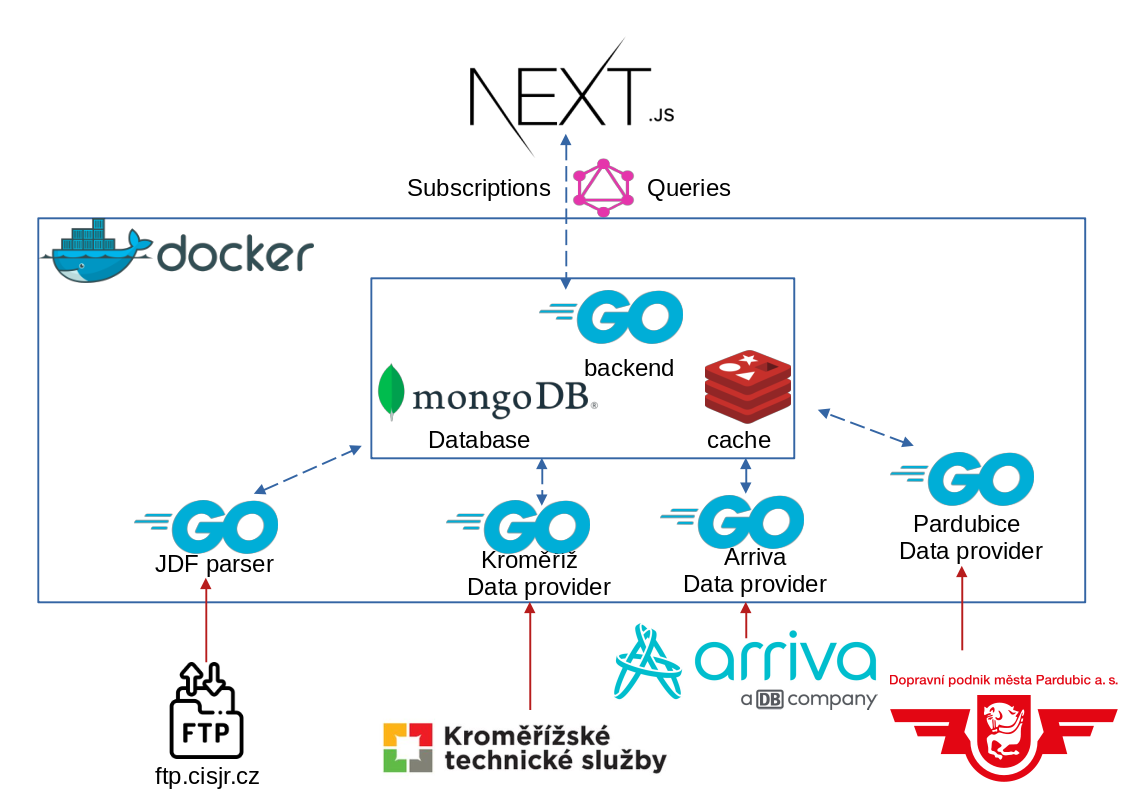
\includegraphics[width=0.75\textwidth]{images/architekturaV5.png}
    \caption{Architektura aplikace}
    \label{architektura}
\end{figure}
\newpage
Tento projekt je rozdělen do~dvou hlavních částí, frontend, vytvořený pomocí frameworku NextJS v programovacím jazyce TypeScript, a~backend, který je napsán v~programovacím jazyce GO.

\section{Backend}

\subsection{Využité technologie}
golang, redis, mongo, docker, graphql, clouflare tunnels
\subsection{několik služeb}
postaveno na micro services, každá služba je samostatným docker kontejnerem
\subsubsection{jednoduchost přidání dalšího dopravce}
modularita
\subsection {komunikace s datovými zdroji}
data jizdnich řadu z cisjr
\subsection {komunikace s jednotlivými podniky}
každý dopravce má svůj vlastní přístup k datům
\subsection {získávání dat spojů}
přiřazení aktuálně jedoucích vozidel k odpovídajícím statickým spojům
\subsection {cache}
cache dat o poloze a nejčastějších spojích a zastávkách
\subsection {graphql}
Subscriptions a query
\subsection{Nasazení na server}

\section{Webová aplikace}

Frontendová část platformy, ve formě webové aplikace a aplikace mobilní je hlavní částí platformy, která živá data o pohybu vozidel komunikuje k cestujícím.

Využívá přitom komunikace s Backendem za pomocí REST + GraphQL API, vše za využití protokolů HTTPS, nebo WebSocket.

Webov

\subsection{Mapa}
Byla vytvořena webová aplikace pro zobrazování aktuálních poloh vozidel dopravních podniků a jiných dopravců.
Na jednotné mapě zobrazujeme všechny dopravce, se kterými spolupracujeme.
Mapu lze ovládat na mobilních zařízeních díky pohybům prsem, nebo na stolních počítačích myší. Podle uživatelského pohledu aplikace vybere dopravce, které by měla zobrazovat a dochází zde k optimalizaci přenášených dat. Do zařízení uživatele jsou přenášeny pouze polohy vozidel, které na mapě vidí.

\subsection{Zobrazování vozidel}
K živému zobrazování dat je třeba několik kroků.

Data jsou nejprve předána z Backendu pomocí GraphQL do aplikace klienta
Z těchto dat je v aplikaci vytvořena plynulá animace pohybu vozidla v reálném čase.
Aplikace využívá interaktivní mapy Leaflet zobrazujeme pro uživatele předpověď pro aktuální pozici vozidel z přijatých dat.
\par
/* obrázek celé mapy */\par
/* obrázek červené cesty spoje i se zastávkami */
\subsection{Cache}
Data prostřednictvím dotazování Backendu jsou na straně cestujícího ukládána do cache, aby již nebylo třeba tato data opakovaně načítat. Cache na straně webové aplikace šetří uživatelům jejich datové připojení a zároveň snižují nároky na vytěžování serveru.

\subsection{Detail spojení}
Pro cestující zpracováváme data o jízdních řádech a nabízíme ve webové aplikaci možnost zobrazit si bližší detail o spojení, které vozidlo právě obsluhuje.

Po stisknutí tlačítka se cestujícímu zobrazí blližší informace o spojení, jako je čas příjezdu k jednotlivým zastávkám spoje, nebo předpokládané zpoždění hlášené dopravcem.
\par
/* obrázek detailnu spojení */
\subsection{Provozní upozornění}
Dopravci mohou přidávat do aplikace klienta provozní upozornění, které se zobrazí v případě, že se vyskytne nějaká situace, která může mít vliv na cestu cestujícího.\par
/* obrázek provozního upozornění */
\subsection{Práce s polohou uživatele}
Aplikace na požádání od uživatele získá jeho aktuální polohu a pro cestujícího v zobrazí zastávky v jeho blízkosti.
/* obrázek aktuální polohy uživatele */
\subsection{Monitorování návštěvnosti}
Zajímavou funkcí pro dopravce je monitorování návštěvnosti aplikace za pomocí Google Analytics. Pro získávání přesných dat o užitečných a oblíbených funkcích aplikace využíváme monitorování vlastních událostí, např. při otevření detailu spoje, nebo vyhledání detailu zastávky.
\subsection{Aplikace a web}
Aplikace využívá experimentálních funkcí nové technologie PWA (Progresivní webové aplikace) jako je například načítání GPS souřadnice uživatele, zobrazování notifikací, nastavení připomínky na přijíždějící spoj.
Funkce PWA zároveň nabízí stahování map do zařízení, aby nemuseli být při každém spuštění znovu stahovány.

Díky technologii PWA je webové aplikaci umožněno využít vnitřního uložiště zařízení pro ukládání dat o mapách, a tím je možné ušetřit uživatelům další stahování a prodlevu před možností využívání aplikace.

\chapter{Bezpečnost}
Webové aplikace jsou v dnešní době rozšířeny do různých odvětví, včetně školství, zdravotnictí a samozřejmě hojně i do běžného života. Toto rozšíření však s sebou nese i rizika kybernetických hrozeb a útoků. Kyberzločinci neustále hledají zranitelná místa ve webových aplikacích, a proto je zabezpečení webových aplikací nezbytnou součástí každého procesu vývoje webových aplikací. \par
Bezpečností webových aplikací se zabývá projekt OWASP (Open Web Application Security Project) se svým seznamem Top 10 nejzávažnějších bezpečnostních rizik webových aplikací. Tento seznam je pravidelně aktualizován, aby odrážel nejnovější trendy v oblasti bezpečnostních hrozeb pro webové aplikace.
\chapter{Závěr}
Závěrem lze říci, že jsme úspěšně vyvinuli platformu, která umožňuje dopravním podnikům měst sdílet data o~poloze v~reálném čase. Díky využití veřejně dostupných dat jízdních řádů, se~podařilo vytvořit spolehlivé a~efektivní řešení pro sdílení údajů o~poloze a~o informacích o~vozidlech veřejné dopravy.\par
Aktuálně je platforma dostupná pro dopravní podniky města Pardubice a.s. (na~adrese \href{https://online.dpmp.cz}{https://online.dpmp.cz}), a~pro technické služby Kroměříž s.r.o \\ (na~adrese \href{https://kromeriz.mhdonline.cz/}{https://kromeriz.mhdonline.cz/}).

V~době psaní této dokumentace probíhá integrace nového dopravce Arriva do~aplikace (na~adrese \href{https://global.mhdonline.cz/}{https://global.mhdonline.cz/})

Plánem do~budoucna je rozšiřovat dostupnost služby i~pro další dopravní podniky v~rámci České republiky.\par
Kromě toho byla platforma navržena s~ohledem na~škálovatelnost a~rozšiřitelnost, což umožňuje budoucí růst a~rozšíření. Celkově tato práce nejen splnila své cíle, ale také prokázala potenciál této platformy výrazně zlepšit komunikaci a~spolupráci s~dopravními podniky.

\begin{thebibliography}{99}
    \bibitem{websocket} \textit{The WebSocket Protocol} [online]. [cit. 2023-03-14]. Dostupné z~\url{https://www.rfc-editor.org/rfc/rfc6455}
    \bibitem{httpVSwebsocket} \textit{Difference between HTTP and WebSocket (HTTP 2.0 )} [online]. https://developerinsider.co/ [cit. 2023-03-19]. Dostupné z~\url{https://developerinsider.co/difference-between-http-and-http-2-0-websocket/}
    \bibitem{framework} \textit{Framework} [online]. [cit. 2023-03-10]. Dostupné z~\url{https://codeinstitute.net/global/blog/what-is-a-framework/}
    \bibitem{jdfpokyn} ČESKÁ REPUBLIKA. METODICKÝ POKYN Č.5 K ORGANIZACI CELOSTÁTNÍHO INFORMAČNÍHO SYSTÉMU O JÍZDNÍCH ŘÁDECH. In: . Ministerstvo dopravy – Odbor veřejné dopravy, 2014, ročník 2014, 11/2014-190-CIS/6. Dostupné také z~\url{https://www.mdcr.cz/getattachment/Dokumenty/Verejna-doprava/Jizdni-rady,-kalendare-pro-jizdni-rady,-metodi-(1)/Jizdni-rady-verejne-dopravy/metodicky-pokyn-cis-5.pdf.aspx}
    \bibitem{cisjr} \textit{Celostátní informační systém o jízdních řádech} CIS JŘ [online]. [cit. 2023-03-12]. Dostupné z~\url{https://portal.cisjr.cz/}
    \bibitem{javascript} \textit{JavaScript} [online]. mozilla.org [cit. 2023-03-19]. Dostupné z~{https://developer.mozilla.org/en-US/docs/Web/JavaScript}
    \bibitem{typescript} \textit{TypeScript} [online]. https://www.typescriptlang.org/ [cit. 2023-03-19]. Dostupné z~\url{https://www.typescriptlang.org/}
    \bibitem{vyhlaskaJizdniRady} ČESKÁ REPUBLIKA. \textit{VYHLÁŠKA ze dne 23. června 2014 o jízdních řádech veřejné linkové dopravy.} In: Sbírka zákonů. 2014, částka 52, číslo 122. Dostupné také z~\url{http://aplikace.mvcr.cz/sbirka-zakonu/ViewFile.aspx?type=z&id=27158}
    \bibitem{chaps} \textit{CHAPS: CIS JŘ} [online]. [cit. 2023-03-13]. Dostupné z~\url{https://www.chaps.cz/cs/products/CIS}
    \bibitem{reactUsers} \textit{The Top Companies That Are Using React Js Services} [online]. [cit. 2023-03-19]. Dostupné z~\url{https://www.bigscal.com/blogs/frontend-technology/top-companies-using-react-js-services-to-their-best/}
    \bibitem{leaflet} \textit{Leaflet} [online]. [cit. 2023-01-25]. Dostupné z~\url{https://leafletjs.com/}
    \bibitem{go} \textit{Go} [online]. [cit. 2023-02-19]. Dostupné z~\url{https://go.dev/}
    \bibitem{graphql} \textit{GraphQL} [online]. [cit. 2023-03-15]. Dostupné z~\url{https://graphql.org/}
    \bibitem{redis} \textit{Redis} [online]. [cit. 2023-03-19]
    \bibitem{docker} \textit{Docker} [online]. [cit. 2023-03-04]. Dostupné z~\url{https://www.docker.com/}
    \bibitem{owasp10} \textit{OWASP Top 10} [online]. [cit. 2023-03-19]. Dostupné z~\url{https://owasp.org/Top10}
    \bibitem{owasp} \textit{OWASP} [online]. [cit. 2023-03-19]. Dostupné z~\url{https://owasp.org/}
    \bibitem{crypto} \textit{Kryptografické selhání} [online]. [cit. 2023-03-19]. Dostupné z~\url{https://owasp.org/Top10/A02_2021-Cryptographic_Failures/}
    \bibitem{animationframe} \textit{MDN Web Docs} [online]. [cit. 2023-03-19]. Dostupné z~\url{https://developer.mozilla.org/en-US/docs/Web/API/window/requestAnimationFrame}
    \bibitem{letsencrypt} \textit{Let's Encrypt} [online]. [cit. 2023-03-19]. Dostupné z~\url{https://letsencrypt.org/}
    \bibitem{pwa} \textit{Wikipedie: Otevřená encyklopedie: Progresivní webové aplikace} [online]. c2023 [citováno 19. 03. 2023]. Dostupný z WWW: \url{https://cs.wikipedia.org/w/index.php?title=Progresivn%C3%AD_webov%C3%A9_aplikace&oldid=22399924>}
    \bibitem{singlepageapp} \textit{HUSP/} [online]. [cit. 2023-03-23]. Dostupné z~\url{https://huspi.com/blog-open/definitive-guide-to-spa-why-do-we-need-single-page-applications/}
    \bibitem{reactlist} \textit{React JS Documentation} [online]. [cit. 2023-03-23]. Dostupné z~\url{https://react.dev/learn/rendering-lists}
    \bibitem{googleanalytics} \textit{Google Cloud Docs} [online]. [cit. 2023-03-24]. Dostupné z~\url{https://cloud.google.com/appengine/docs/flexible/integrating-with-analytics?tab=node.js#top}
    \bibitem{magiclinklogin} \textit{WorkOS} [online]. [cit. 2023-03-24]. Dostupné z~\url{https://workos.com/blog/a-guide-to-magic-links}
    \bibitem{nosqlinjection} \textit{Testing for NoSQL Injection} [online]. [cit. 2023-03-24]. Dostupné z~\url{https://owasp.org/www-project-web-security-testing-guide/latest/4-Web_Application_Security_Testing/07-Input_Validation_Testing/05.6-Testing_for_NoSQL_Injection}
\end{thebibliography}

\end{document}